\begin{figure}[!htb]
\centering
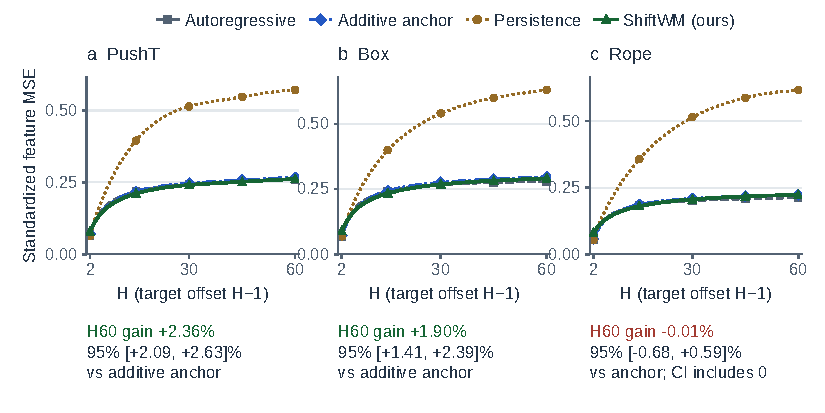
\includegraphics[width=\linewidth]{generated/experiment_alignment/forecast_transfer.pdf}
\caption[Single-observation IWS development forecasts.]{\textbf{Single-observation IWS development forecasts.} Each curve retains all 59 future offsets from one observed image and the corresponding causal command prefix. The horizontal axis is $H=2,\ldots,60$, whose target is stored offset $H-1$, not physical time. Native training-standardized feature MSE averages windows within trajectory, then trajectories and three matched seeds equally; lower is better. Each task has its own zero-based vertical scale. Annotations give signed relative $H=60$ MSE reduction versus the learned additive anchor and the registered paired 95\% seed--trajectory interval; positive values favor ShiftWM. Intervals are unadjusted exploratory comparisons, with no invented uncertainty bands on the curves. All three tasks, all three learned arms and persistence are retained. Reserved upstream-validation evaluation is separate.}
\label{fig:iws-forecast-transfer}
\end{figure}
